\section{Технический проект}
\subsection{Общая характеристика организации решения задачи}

Необходимо спроектировать и разработать базу данных для корпоративного мессенджера, которая должна обеспечивать надежное хранение и быстрый доступ к сообщениям, пользовательским данным и информации о группах.

База данных представляет собой структурированный набор взаимосвязанных таблиц, содержащих текстовую информацию (сообщения, имена пользователей), метаданные (временные отметки, идентификаторы) и системные данные (роли, статусы). База располагается в файле data.db и использует SQLite в качестве системы управления.

\subsection{Обоснование выбора технологии проектирования}

Для реализации корпоративного мессенджера рассмотрены различные СУБД, включая PostgreSQL, MySQL и SQLite. Выбор SQLite обусловлен следующими факторами:

\subsubsection{Система управления базами данных SQLite}

SQLite — встраиваемая реляционная СУБД, не требующая отдельного серверного процесса. Основные преимущества в контексте проекта:

\begin{itemize}
	\item нулевая конфигурация — не требует администрирования;
	\item компактность — вся база в одном файле;
	\item высокая производительность для операций чтения/запись;
	\item полная поддержка транзакций ACID.
\end{itemize}

\subsubsection{Достоинства SQLite для данного проекта}
\begin{itemize}
	\item идеально подходит для приложений с одним пользователем или небольших рабочих групп;
	\item не требует отдельного сервера БД, что упрощает развертывание;
	\item поддерживает большинство возможностей SQL-92.
\end{itemize}

\subsubsection{Ограничения SQLite}
\begin{itemize}
	\item ограниченная поддержка одновременных записей (write-ahead logging включен);
	\item максимальный размер базы данных около 140 TB (достаточно для корпоративного мессенджера);
	\item отсутствие встроенной системы аутентификации пользователей.
\end{itemize}

\subsection{Диаграмма компонентов базы данных}

Диаграмма компонентов базы данных представляет собой визуализацию структуры и взаимосвязей основных модулей системы хранения данных.

\begin{figure}[ht]
\center{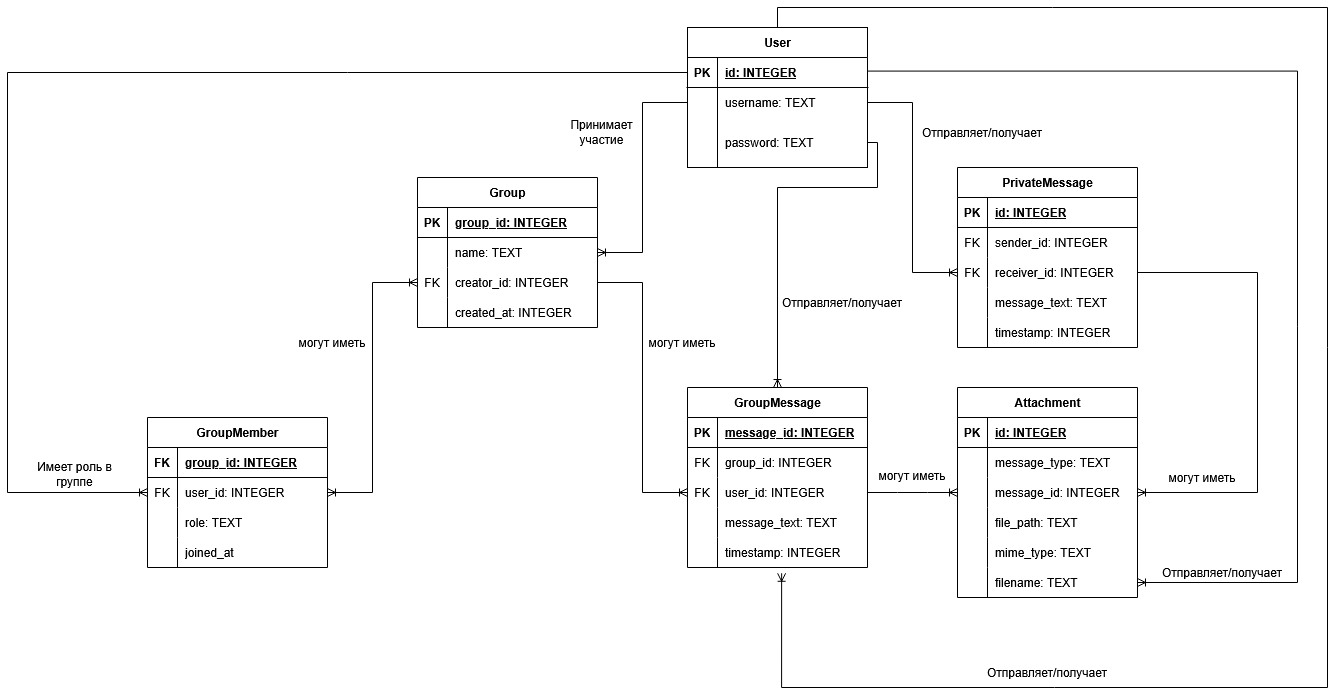
\includegraphics[width=1\linewidth]{ЕР модель}}
\caption{Диаграмма компонентов базы данных}
\label{comp:image}
\end{figure}

ER-модель отражает строгую структуру данных, построенную вокруг взаимодействия пользователей в групповых и приватных чатах. В центре системы находится сущность "Пользователь", хранящая учетные данные и выступающая отправителем сообщений. Группы организуют коллективное общение, фиксируя создателя и время создания, а Сообщения делятся на групповые и приватные, с обязательной привязкой к отправителю и временной меткой.

Система ролей реализована через связующую сущность "GroupMember", которая определяет права участников групп (владелец, администратор, участник) и дату их присоединения. Это обеспечивает гибкое управление доступом внутри чатов. Для работы с файлами используется сущность "Attachment", привязанная к сообщениям и содержащая технические данные о файлах (путь, тип, оригинальное имя), что позволяет единообразно обрабатывать вложения как в групповых, так и в личных сообщениях.

Модель подчеркивает важность целостности данных через систему внешних ключей, гарантируя, что сообщения не могут существовать без отправителя или чата. Поле "timestamp" обеспечивает учет активности пользователей, а минималистичная реализация приватных чатов (прямая связь отправитель-получатель) упрощает архитектуру. Вынос вложений в отдельную таблицу позволяет менять способ хранения файлов без изменения структуры сообщений.

\subsection{Таблицы базы данных}
\subsubsection{User - Пользователи системы}
\begin{xltabular}{\textwidth}{|l|l|X|}
	\caption{Атрибуты сущности "Пользователи"\label{user:table}}\\ \hline
	\centrow Поле & \centrow Тип & \centrow Описание \\ \hline
	\thead{id} & \thead{INTEGER} & Первичный ключ (PK), уникальный идентификатор пользователя \\ \hline
	\thead{username} & \thead{TEXT} & Имя пользователя (уникальное) \\ \hline
	\thead{password} & \thead{TEXT} & Хэшированный пароль пользователя \\ \hline
\end{xltabular}

Таблица "User" хранит информацию о зарегистрированных пользователях мессенджера. Каждый пользователь имеет уникальный идентификатор, имя пользователя и пароль. Является центральной сущностью системы, с которой связаны все остальные таблицы.

\subsubsection{Group - Групповые чаты}
\begin{xltabular}{\textwidth}{|l|l|X|}
	\caption{Атрибуты сущности "Групповые чаты"\label{group:table}}\\ \hline
	\centrow Поле & \centrow Тип & \centrow Описание \\ \hline
	\thead{group\_id} & \thead{INTEGER} & Первичный ключ (PK), ID группы \\ \hline
	\thead{name} & \thead{TEXT} & Название группы \\ \hline
	\thead{creator\_id} & \thead{INTEGER} & Внешний ключ (FK→User), ID создателя группы \\ \hline
	\thead{created\_at} & \thead{INTEGER} & Timestamp создания группы \\ \hline
\end{xltabular}

Таблица "Group" содержит информацию о групповых чатах. Каждая группа имеет уникальный идентификатор, название, создателя и время создания. Создатель группы автоматически становится владельцем (owner).

\subsubsection{GroupMember - Участники групп с ролями}
\begin{xltabular}{\textwidth}{|l|l|X|}
	\caption{Атрибуты сущности "Участники групп"\label{groupmember:table}}\\ \hline
	\centrow Поле & \centrow Тип & \centrow Описание \\ \hline
	\thead{group\_id} & \thead{INTEGER} & Внешний ключ (FK→Group), ID группы \\ \hline
	\thead{user\_id} & \thead{INTEGER} & Внешний ключ (FK→User), ID пользователя \\ \hline
	\thead{role} & \thead{TEXT} & Роль в группе: 'owner' (владелец), 'admin' (администратор), 'member' (участник) \\ \hline
	\thead{joined\_at} & \thead{INTEGER} & Timestamp вступления пользователя в группу \\ \hline
\end{xltabular}

Таблица "GroupMember" определяет состав участников групп и их роли. Реализует систему прав доступа, аналогичную Telegram, где владелец имеет максимальные права, администраторы - ограниченные права управления, а участники - базовые права.

\subsubsection{GroupMessage - Сообщения в группах}
\begin{xltabular}{\textwidth}{|l|l|X|}
	\caption{Атрибуты сущности "Групповые сообщения"\label{groupmessage:table}}\\ \hline
	\centrow Поле & \centrow Тип & \centrow Описание \\ \hline
	\thead{message\_id} & \thead{INTEGER} & Первичный ключ (PK), ID сообщения \\ \hline
	\thead{group\_id} & \thead{INTEGER} & Внешний ключ (FK→Group), ID группы \\ \hline
	\thead{user\_id} & \thead{INTEGER} & Внешний ключ (FK→User), ID отправителя \\ \hline
	\thead{message\_text} & \thead{TEXT} & Текст сообщения (может быть пустым для сообщений с вложениями) \\ \hline
	\thead{timestamp} & \thead{INTEGER} & Время отправки сообщения (timestamp) \\ \hline
\end{xltabular}

Таблица "GroupMessage" хранит все сообщения, отправленные в групповых чатах. Каждое сообщение связано с группой и пользователем-отправителем. Поддерживает текстовые сообщения и сообщения с вложениями (через таблицу Attachment).

\subsubsection{PrivateMessage - Личные сообщения}
\begin{xltabular}{\textwidth}{|l|l|X|}
	\caption{Атрибуты сущности "Личные сообщения"\label{privatemessage:table}}\\ \hline
	\centrow Поле & \centrow Тип & \centrow Описание \\hline
	\thead{id} & \thead{INTEGER} & Первичный ключ (PK), уникальный идентификатор сообщения \\ \hline
	\thead{sender\_id} & \thead{INTEGER} & Внешний ключ (FK→User), ID отправителя сообщения \\ \hline
	\thead{receiver\_id} & \thead{INTEGER} & Внешний ключ (FK→User), ID получателя сообщения \\ \hline
	\thead{message\_text} & \thead{TEXT} & Текст сообщения (может быть пустым для сообщений с вложениями) \\ \hline
	\thead{timestamp} & \thead{INTEGER} & Время отправки сообщения (timestamp) \\ \hline
\end{xltabular}

Таблица "PrivateMessage" хранит историю приватных сообщений между пользователями. Каждое сообщение связывает отправителя и получателя, поддерживает текстовый контент и вложения (через таблицу Attachment). Реализует функционал личной переписки между сотрудниками организации.

\subsubsection{Attachment - Вложения к сообщениям}
\begin{xltabular}{\textwidth}{|l|l|X|}
	\caption{Атрибуты сущности "Вложения"\label{attachment:table}}\\ \hline
	\centrow Поле & \centrow Тип & \centrow Описание \\ \hline
	\thead{id} & \thead{INTEGER} & Первичный ключ (PK), уникальный идентификатор вложения \\ \hline
	\thead{message\_type} & \thead{TEXT} & Тип сообщения: 'general' (системные), 'group' (групповые), 'private' (личные) \\ \hline
	\thead{message\_id} & \thead{INTEGER} & ID сообщения, к которому относится вложение \\ \hline
	\thead{file\_path} & \thead{TEXT} & Путь к файлу в файловом хранилище системы \\ \hline
	\thead{mime\_type} & \thead{TEXT} & MIME-тип файла для корректной обработки клиентом \\ \hline
	\thead{filename} & \thead{TEXT} & Оригинальное имя файла для отображения пользователю \\ \hline
\end{xltabular}

Таблица "Attachment" обеспечивает хранение файловых вложений для всех типов сообщений в системе. Универсальная структура позволяет прикреплять файлы к групповым чатам, личным сообщениям и системным уведомлениям. Содержит метаданные файлов для правильного отображения в клиентских приложениях.

На рисунке \ref{data:image} представлена схема обмена данными между сценариями компонента при вызове компонента на странице сайта.

\begin{figure}[H]
\center{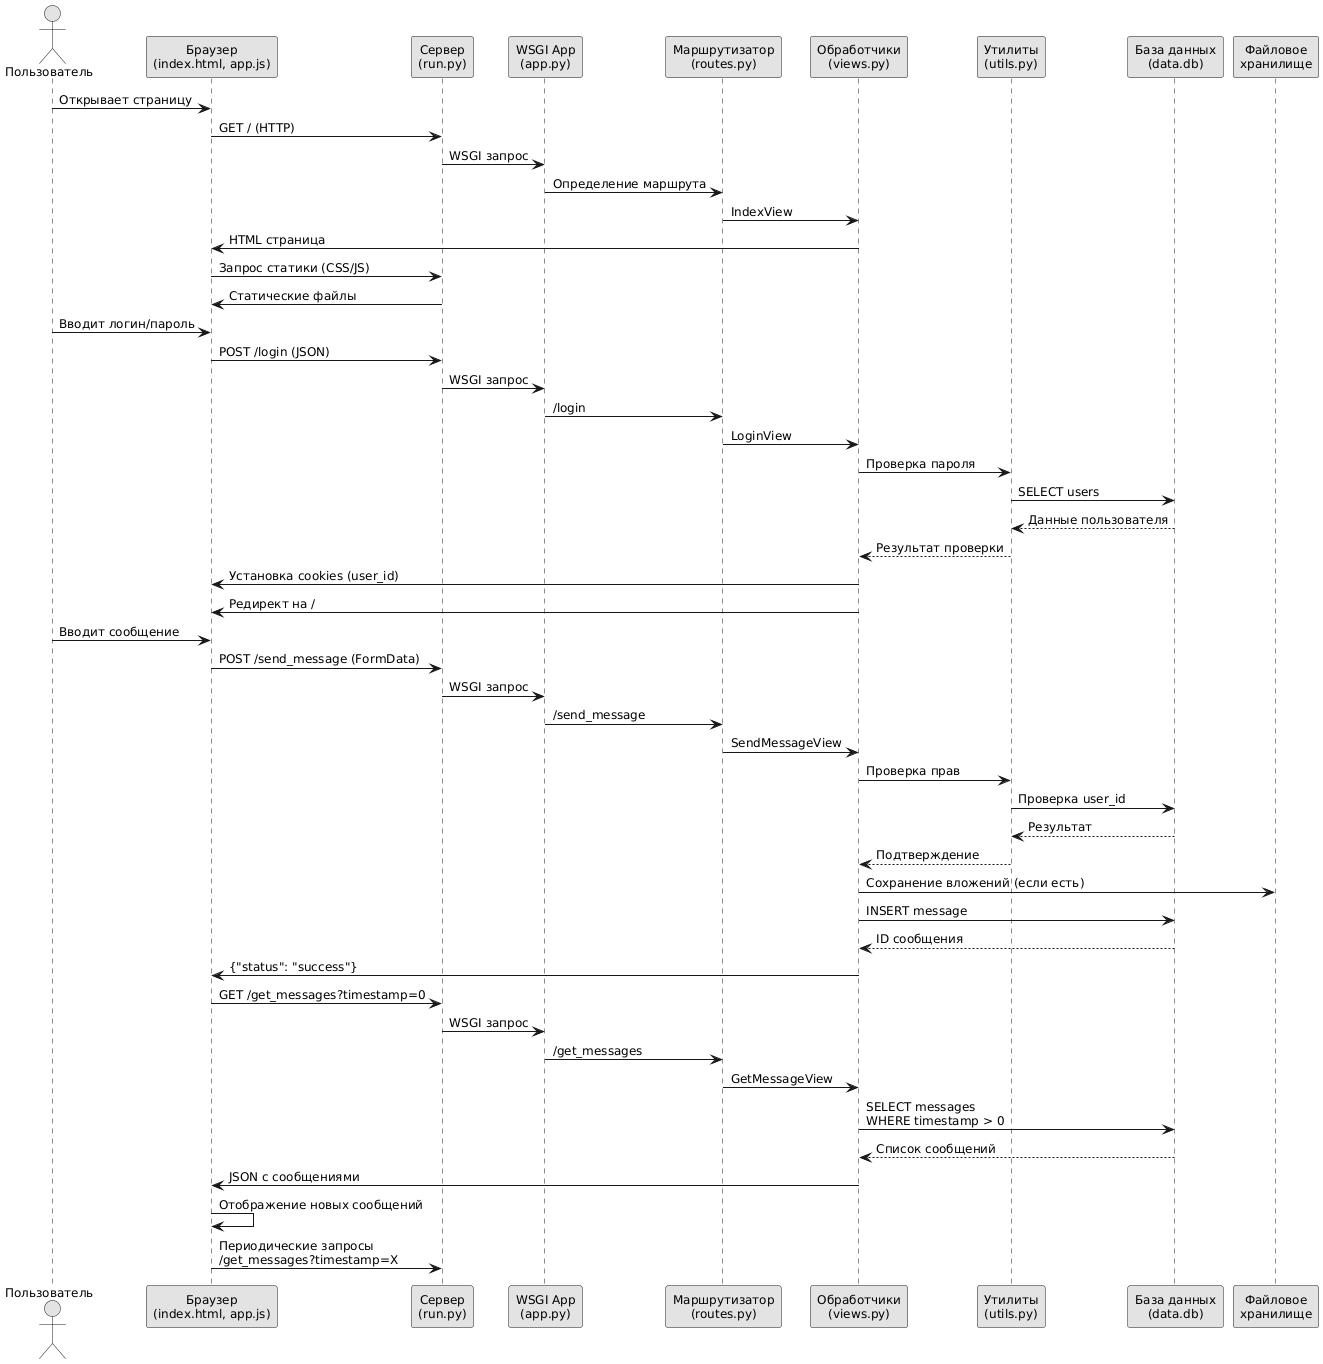
\includegraphics[width=1\linewidth]{Диаграмма последовательности}}
\caption{Диаграмма компонентов}
\label{data:image}
\end{figure}

\subsection{Описание диаграммы последовательности работы корпоративного мессенджера}

\begin{enumerate}[leftmargin=*,label=\textbf{\arabic*.}]
	\item \textbf{Загрузка страницы (инициализация)}
	\begin{itemize}
		\item пользователь открывает в браузере главную страницу (\texttt{index.html});
		\item браузер отправляет HTTP GET-запрос на сервер;
		\item серверный скрипт \texttt{run.py} (Waitress) получает запрос;
		\item запрос передаётся в WSGI-приложение (\texttt{app.py});
		\item маршрутизатор (\texttt{routes.py}) определяет обработчик \texttt{IndexView};
		\item пользователю возвращается HTML-страница и статические файлы (CSS/JS).
	\end{itemize}
	
	\item \textbf{Процесс аутентификации}
	\begin{itemize}
		\item пользователь вводит логин и пароль в форму входа;
		\item браузер отправляет POST /login запрос (JSON);
		\item \texttt{LoginView} проверяет учётные данные:
		\begin{itemize}
			\item через \texttt{utils.py} выполняется SQL-запрос к таблице \texttt{users};
			\item пароль проверяется с помощью bcrypt.
		\end{itemize}
		\item при успешной аутентификации:
		\begin{itemize}
			\item устанавливается cookie с \texttt{user\_id}
			\item происходит редирект на главную страницу.
		\end{itemize}
	\end{itemize}
	
	\item \textbf{Отправка нового сообщения}
	\begin{itemize}
		\item пользователь вводит текст и/или прикрепляет файлы;
		\item браузер формирует FormData и отправляет POST /send\_message;
		\item \texttt{SendMessageView} выполняет:
		\begin{itemize}
			\item проверку прав через cookies;
			\item сохранение файлов в \texttt{static/uploads};
			\item запись сообщения в БД (таблицы \texttt{messages} или \texttt{group\_messages});
		\end{itemize}
		\item клиент получает JSON с результатом операции;
	\end{itemize}
	
	\item \textbf{Получение сообщений (реализация чата)};
	\begin{itemize}
		\item браузер периодически опрашивает сервер (GET /get\_messages);
		\item \texttt{GetMessageView} запрашивает новые сообщения из БД;
		\item сервер возвращает JSON с массивом сообщений;
		\item браузер динамически обновляет интерфейс чата;
	\end{itemize}
	
	\item \textbf{Особенности работы}
	\begin{itemize}
		\item все запросы проходят через единую точку входа (\texttt{app.py});
		\item маршрутизатор выбирает соответствующий View-класс;
		\item бизнес-логика сосредоточена во \texttt{views};
		\item работа с БД вынесена в \texttt{utils.py};
		\item файлы хранятся локально в файловой системе;
		\item состояние сессии поддерживается через cookies.
	\end{itemize}
\end{enumerate}

\subsection{Диаграмма размещения}

Диаграмма размещения (рис.~\ref{place:image}) отражает физические взаимосвязи между программными и аппаратными компонентами системы.

\begin{figure}[ht]
\center{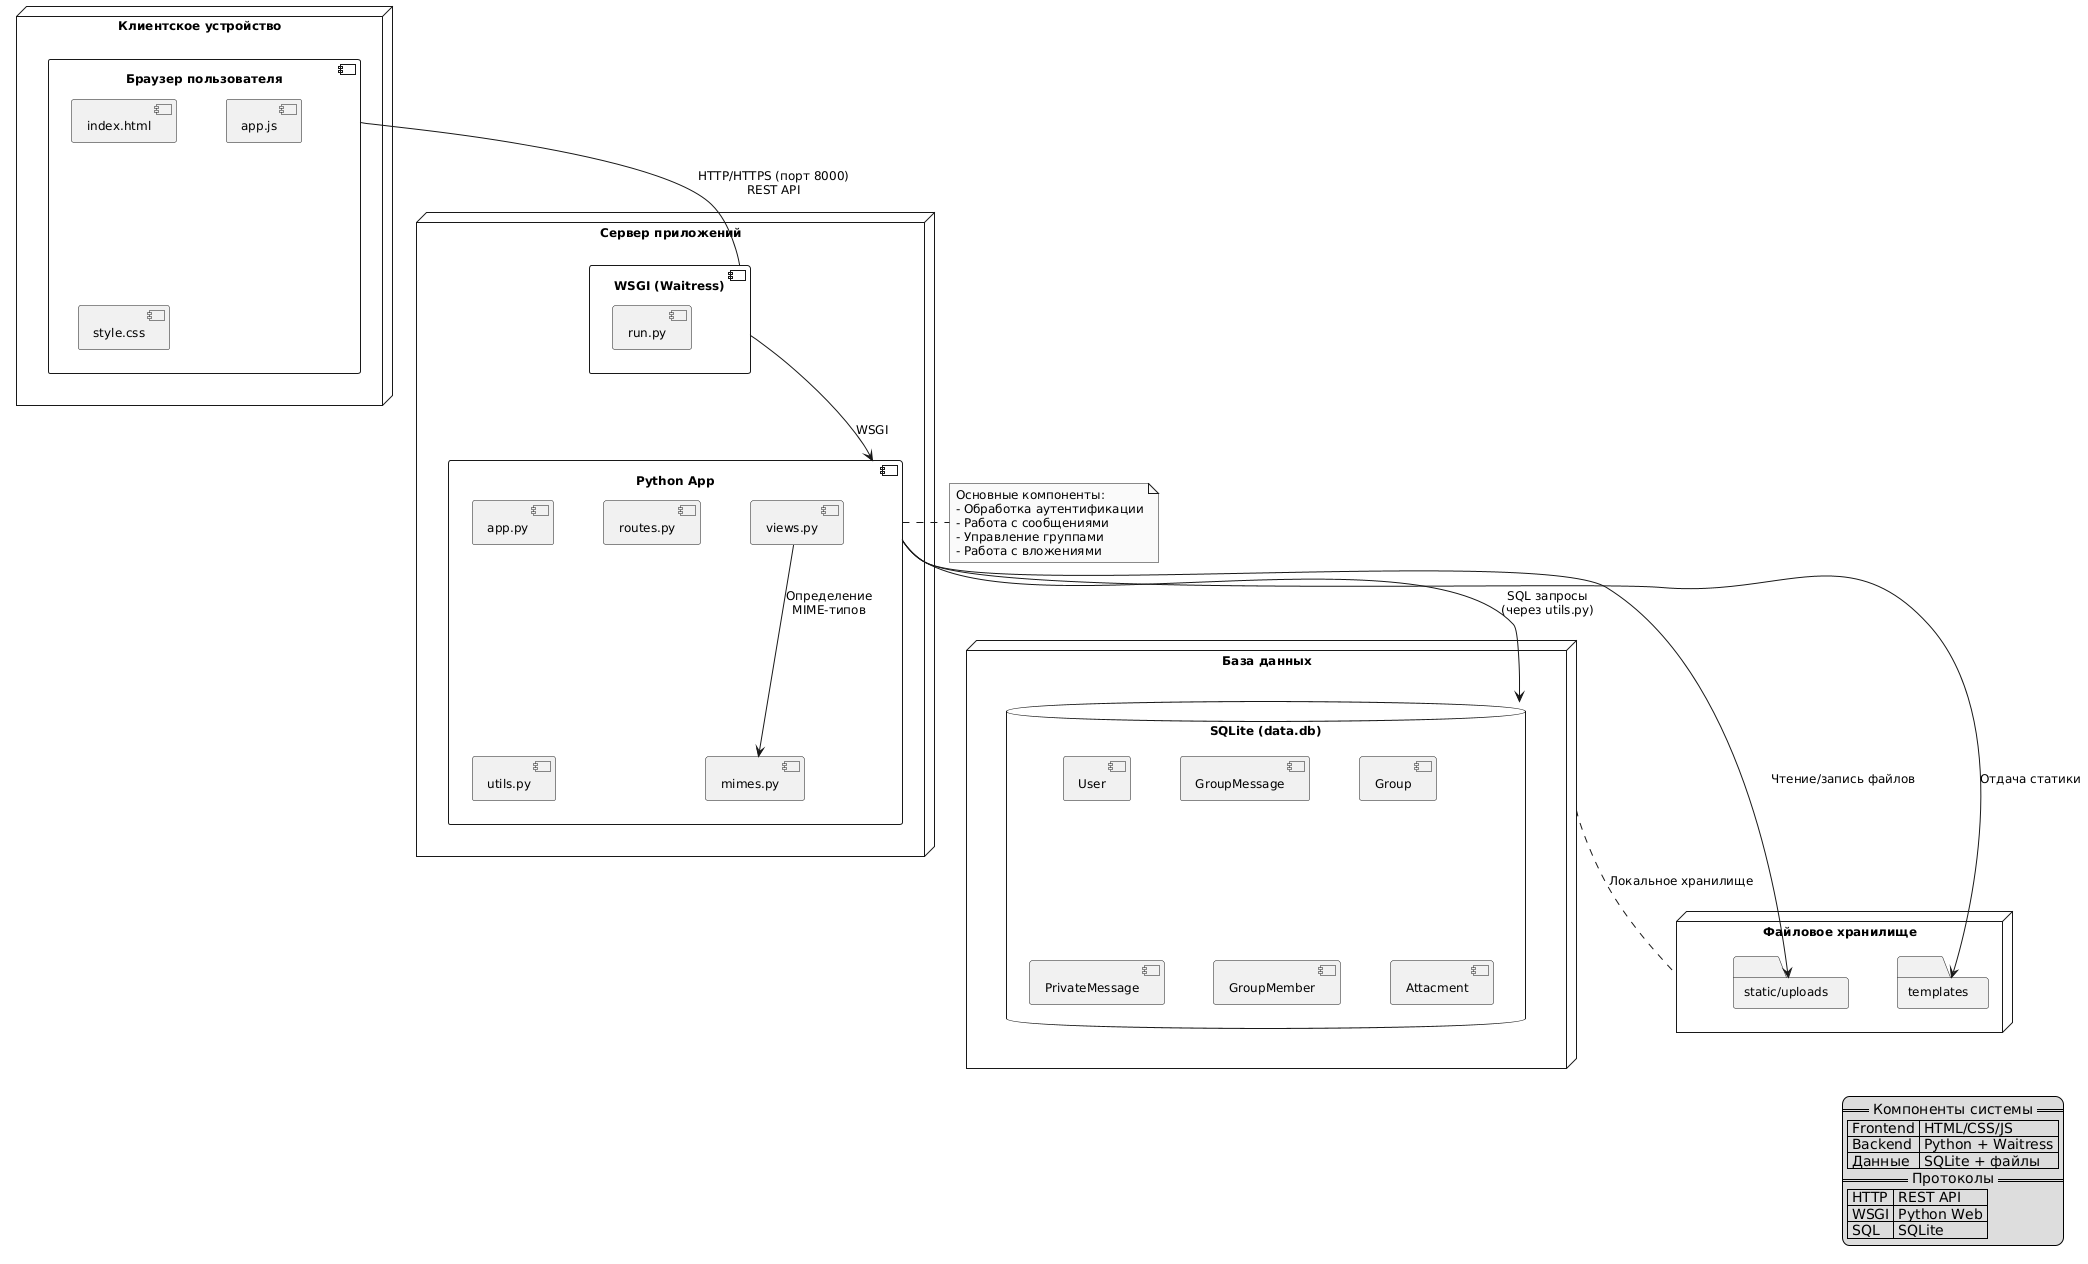
\includegraphics[width=1\linewidth]{Диаграмма развёртывания}}
\caption{Диаграмма развёртывания}
\label{place:image}
\end{figure}

Диаграмма развертывания отображает архитектуру корпоративного мессенджера. На стороне клиента взаимодействие с системой осуществляется через веб-браузер, который загружает статические файлы интерфейса — HTML-шаблоны, JavaScript-код и CSS-стили.

Серверная часть реализована на Python с использованием WSGI-сервера Waitress, обрабатывающего входящие HTTP-запросы на порту 8000. Логика приложения организована в виде пакетов views и models. Пакет views содержит специализированные модули для обработки запросов: auth.py отвечает за аутентификацию, groups.py управляет групповыми чатами, message.py обрабатывает сообщения, p\_chat.py обеспечивает личную переписку. Пакет models включает UserModel.py, GroupModel.py и MessageModel.py, инкапсулирующие работу с данными. Вспомогательные функции вынесены в utils.py и mimes.py.

Хранение данных организовано в двух форматах. Реляционная база SQLite (файл data.db) содержит таблицы User, Group, GroupMember, GroupMessage, PrivateMessage и Attachment, обеспечивающие хранение структурированной информации о пользователях, чатах, сообщениях и вложениях. Файловое хранилище в папках static/uploads и templates обслуживает медиафайлы и шаблоны интерфейса.

Взаимодействие между компонентами осуществляется через API между клиентом и сервером. WSGI-сервер передает запросы в Python-приложение, где они обрабатываются соответствующими модулями пакета views. Для работы с данными views используют методы пакета models, которые выполняют SQL-запросы к базе данных. Файловые вложения передаются напрямую через специальные обработчики.

Архитектура системы сохраняет принцип самодостаточности — все компоненты развертываются на едином сервере без внешних зависимостей. Четкое разделение на модули views и models обеспечивает безопасность и упрощает дальнейшее развитие системы, сохраняя при этом возможность автономной работы в корпоративной сети.

